%!TEX root = Constructive Alignment for Introductory Programming.tex

\chapter{Approaching Constructive Alignment with Portfolio Assessment} % (fold)
\label{cha:approach}

\graphicspath{{Figures/CAApproach/}}

\cref{cha:guiding_principles} outlined nine principles for guiding \emph{how} to teach introductory programming, and three principles for \emph{what} should be taught. This chapter proposes a model for applying constructive alignment for teaching introductory programming.

\section{Assessment Strategy} % (fold)
\label{sec:assessment_strategy}

One of the overarching principles from \cref{cha:guiding_principles} was the requirement to be agile and willing to change (\pref{itm:agile}). In discussing this principle, \sref{ssub:be_agile_and_willing_to_change} outlines that teaching and learning resources need to be guided by an overall strategy. This strategy informs, and is shaped by, the assessment approach. 

Assessment plays an important role in defining what students learn. \citet{Rowntree:1977} indicated the central role of assessment procedures in understanding any education system. This is supported by \citet{Ramsden:2003}, who stated that ``from our students' point of view, assessment always defines the actual curriculum'', and further supported by \citet{Biggs:2007} who indicated that ``students learn what they \emph{thing} they will be tested on''. In presenting their conditions for effective assessment, \citet{Gibbs:2004} discussed the dominant influence of assessment in defining what students focus on, indicating that students are able to distinguish between what assessment requires them to pay attention to and what is likely to result in effective learning. So the selection of an assessment approach will have a significant impact on the overall strategy for both students and staff. 

Traditionally introductory programming was taught using a number of assignments and a final examination. This approach, while commonly used, is not in keeping with several of our guiding principles. The use of summative assessment during the semester goes against \pref{itm:formative} with its goal of assessing outcomes. The use of assignments to motivate students is also contrary to \pref{itm:theory_y}, with marks being used for motivation in either a hard or soft form of Theory X strategy. These principles required us to examine other forms of assessment.

One strategy to address this would be to consider abandoning coursework assignments, delay final summative assessment to an examination worth 100\% of the student's grade. While this would address \pref{itm:formative}, such a heavy weight examination is very much a hard Theory X approach. The value of coursework assignments was strongly argued for in \citet{Gibbs:2004}. This work provided several strong arguments for coursework assignments, including the following:
\begin{itemize}[noitemsep,nolistsep]
	\item Students attain better results from coursework than examinations, referring to their Gibbs' earlier work that indicated a strong positive correlation between proportion of coursework and average marks.
	\item Students prefer coursework assignments over examinations. A position that is supported by \citet{Kniveton:1996} who stated that students prefer coursework assignments to exams as assignments assessed a better range of their abilities and enabled them to organise their time to a greater extent.
	\item Coursework assignments are at least as valid a form of assessment as examinations:
	\begin{itemize}
		\item Exams are a poor predictor of future performance.
		\item Coursework assignments are a better predictor of long term learning than exam results \cite{Conway:1992}. This supports the idea that students adopt surface approaches to preparing for exams \citet{Marton:1976a}. 
		\item The quality of learning is higher in assignment-based units, when compared to exam-based units.
	\end{itemize}
\end{itemize}

The challenge, therefore, is to define an assessment approach that enables students to construct their knowledge, uses coursework assignments in a formative manner, and enables 100\% of the students grade to be determined after the end of the teaching period.

\subsection{Portfolio Assessment} % (fold)
\label{sub:portfolio_assessment}

In proposing Constructive Alignment, \citet{Biggs:1996c} advocated strongly for the use of an assessment portfolio, and indicated that the principles of constructive alignment had evolved with the decision to use portfolio assessment. This work was extended in \cite{Biggs:1997} which outlined suggestions for implementing portfolio assessment and a generalised model for instruction design. Further advice and details of the generalised model were presented in \citet{Biggs:2007} text on quality learning at university.

Assessment involves three components, all of which are typically under the control of the teacher \cite{Biggs:1997}. These include \emph{setting criteria}, \emph{selecting evidence} and \emph{making a judgement}. With the assessment portfolio the students take control of at least the selection of evidence. The portfolio is then a collection of work that the student puts forward for assessment against the unit's intended learning outcomes.

\citet{Smith:2001,Smith:2003} identified four different kinds of portfolios evident in the research literature: dossier, reflective, training and personal development. These reflected the combination of two factors: the purpose of the portfolio as either for selection/promotion or learning, and whether the portfolio is self-directed or mandated. The details of these are described in the following list, and shown in \fref{fig:portfolio_types}.

\begin{description}[noitemsep,nolistsep]
	\item[Dossier] is a portfolio for the purpose of selection or promotion that contains a mandated collection of work to demonstrate achievement. (selection/promotion, mandated)
	\item[Reflective] portfolios contain a self selected collection of work that demonstrates growth or accomplishment for the purpose of admission or promotion. The portfolio is accompanied by a self-appraisal, with the justification for the selection of pieces being as important as the evidence itself. (selection/promotion, self-directed)
	\item[Training] portfolios are a mandated collection of work performed in a learning context. The portfolio has a fixed format, and contains representative work from the student demonstrating acquired skills, knowledge and competencies. (learning, mandated)
	\item[Personal development] portfolios are a self selected collection of work, and reflective account of personal growth over an extended period. (learning, self-directed)
\end{description}

\begin{figure}[htbp]
	\centering
	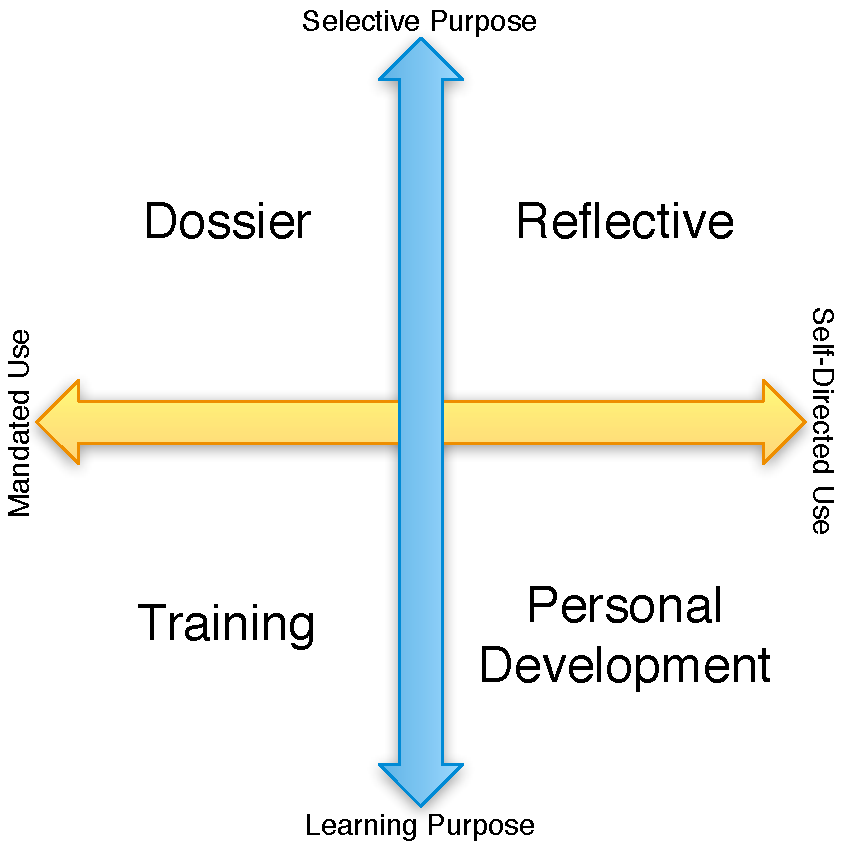
\includegraphics[width=0.50\textwidth]{PortfolioTypes}
	\caption{The four kinds of portfolio based upon purpose and use from \citet{Smith:2001}.}
	\label{fig:portfolio_types}
\end{figure}

Biggs' use of an \emph{assessment portfolio} clearly fits with the \emph{Training} portfolio classification, being a mandated part of the unit assessment for the purpose of evaluating learning outcomes. In the study of a small group of professionals, \citet{Smith:2001} found the training portfolio to be highly rated. Their findings indicated that students found the training portfolio confusing initially, but that once they had understood its function and rational they liked the approach, were easily able to construct their portfolio, and felt it was a fair way to assess their learning.

\citet{Tang:1999} provides further evidence of the value of portfolio assessment. In evaluating how students approach study, \citet{Tang:1999} found that students tended to have a narrow, surface approach to studying for tests. These same students were found to adopt wider, more cognitively challenging, approaches when preparing for a portfolio assessment. 

Portfolio assessment enables the shift from Theory X ``sage on the stage'' views to a Theory Y ``guide by the side'' view. The traditional approach of setting assignments and exams in which educators test student ability becomes inverted with portfolio assessment. With portfolio assessment it is the students responsibility to demonstrate how they have met the unit's intended learning outcomes. This frees educators to help students and to guide them in the preparation of their evidence. We are now working side by side with the students, helping them to achieve the intended learning outcomes.

Portfolio assessment appears to align well with all nine ``\emph{how}'' principles listed in \cref{cha:guiding_principles}. 
\begin{enumerate}[noitemsep,nolistsep]
	\item The portfolio consists of a collection of work the student feels demonstrates the depth of their knowledge. (\Pref{itm:construct})
	\item Assessment criteria for the portfolio can be aligned with the unit's intended learning outcomes. (\Pref{itm:align})
	\item The portfolio can be used as the sole form of summative assessment, with students being able to take advantage of formative feedback throughout the teaching period. (\Pref{itm:formative})
	\item A focus on depth will ensure the portfolio requires students to engage high cognitive levels, requiring them to explain, justify and reflect. (\Pref{itm:depth})
	\item By communicating high expectations, students will strive to create high quality evidence for their portfolios. (\Pref{itm:expectations})
	\item Students will develop evidence for their portfolio from day 1, everything they do could be of potential value. This will require active support from teaching staff. (\Pref{itm:support})
	\item Without marks for motivation, an entirely portfolio assessed unit empowers students in the learning process, and must trust that they are able to effectively manage their own learning. (\Pref{itm:theory_y})
	\item Portfolio assessment, with frequent formative feedback, is very much akin to agile software development processes. In addition, student portfolios will provide a wealth of evidence to help guide change. (\Pref{itm:agile})
	\item Incorporating a reflective component in the portfolio will encourage students to engage in reflective practice. (\Pref{itm:reflect})
\end{enumerate}

% subsection portfolio_assessment (end)


% section assessment_strategy (end)



% chapter approaching_constructive_alignment_with_portfolio_assessment (end)